% !TeX root = main.tex
\chapter{Paper-based semantic speech editing}\label{chp:paper-based}

\section{Introduction}

Digital documents are often reviewed and proofread by printing the document and using a pen to annotate the text. This
approach is still popular, despite the widespread availability of similar functionality in word processors
\citep{Harper2001}.

Working on paper offers a number of advantages over working on computer.  Paper is lightweight, portable and does not
require any power, which allows readers to work anywhere.  It is not back-lit, so is easier on the eyes.
%It can be annotated freely whilst reading.
It can be navigated quickly, annotated freely whilst reading and individual pages can be laid out and easily compared.
Its physical low-tech nature also means that it is intuitive, robust, durable and does not crash or lose data.  These
advantages mean that reading from paper rather than a screen allows readers to gain a deeper understanding, easily
cross-reference other documents, and interleave reading and writing \citep{OHara1997}.

%Transcripts are often printed out because:
%- it is easier to read than on screen
%- allows portability,
%- allows annotation,
%- flexible spatial layout
%- quick navigation
%- cross-referencing,
%- reduces battery anxiety,
%- more trusted by non-tech-savvy users

A similar process happens in the production of media content. The production workflow typically involves recording
material, selecting which parts of that material to use, then editing the desired material down to the final output
\citep{Baume2015}.  Many producers will `log' the material after it is recorded by writing transcripts of what was
said.  This is either done themselves or using a third-party service. These transcripts help producers to recall what
was said and when, identify themes, and make links between different parts of their content.

Many producers find this process easier to achieve on paper than directly on the screen, so choose to print the
transcript. The producer makes hand-written annotations to help them structure their program and make editorial
decisions.  After they have decided which parts they want to use in their programme, they must use audio or video
editing software to manually execute these editorial decisions, which is a tedious and slow process.

In this paper, we describe a system which allows users to edit audio and video content directly using a printed
transcript.  Speech-to-text is used to generate a transcript that has precise timestamps for each word.  The transcript
is printed with an Anoto dot-pattern \citep{Fahraeus2003}, which allows a compatible digital pen to capture annotations
make on the paper.  A digital pen is used to annotate the transcript to mark which parts of the transcript the user
wants to keep or remove.  The audio or video content is then automatically edited to reflect the annotations made on
the transcript.

%The producer prints the transcript then uses
%a digital pen to highlight and strikethrough words to signify the parts they
%want or don't want (see Figure~\ref{fig:layout}). These marks are then
%automatically translated into edit commands by using the timestamps of the
%words to calculate the in-- and out-points for each cut. This produces an edit
%decision list which can be opened in an audio or video editor.

%In this paper, we describe a system which allows users to edit audio and video
%content directly using a printed transcript. Speech-to-text is used to extract
%a transcript with precise timings for each word.
%The digital pen is used
%to select or delete parts of the transcript.

%Our system automatically generates a transcript using speech-to-text. Even
%though it's imperfect, it is good enough to make edit decisions with
%\citep{Whittaker2004}

\section{Related work}
Our system combines editing of media using transcripts with annotation of paper using digital pens. These approaches
have previously been explored individually, alongside related techniques such as navigation of media using paper
transcripts, digital ink annotation of video and paper-based note taking for media.

Transcript-based interfaces have already successfully been applied to both audio and video editing. SCANMail
\citep{Whittaker2002} demonstrated the advantages of navigating voicemail recordings using a transcript, but did not
include editing capabilities.  The LIDS Editor \citep{Apperley2002}, and later TRAED \citep{Masoodian2006}, used
automatically-generated transcripts to allow users to navigate and edit lecture recordings by removing and rearranging
sentences and words. Even though automatically-generated transcripts are imperfect, Whittaker and Amento found they are
sufficiently accurate to allow navigation and editing \citep{Whittaker2004}.  More recently, Rubin \citep{Rubin2013}
created a system for using editable crowd-sourced transcripts to create audio stories.  Similar techniques have been
applied to video editing. SILVER \citep{Casares2002} was a video editor that had an editable transcript window,
generated from subtitles, and Berthouzoz et. al.  \citep{Berthouzoz2012} developed a system that used crowd-sourced
transcripts and image processing to allow text-based editing of multi-camera video interviews.

The Anoto dot pattern can be used with digital pens to bridge the gap between paper and digital documents. PADD
\citep{Guimbretiere2003} was a concept for a system of editing documents that allowed users to move from digital to
paper and back again. ProofRite \citep{Conroy2004} was an implementation of this, which anchored annotations made on
paper into a word processor such that they `reflow' with the text they were attached to.  PaperProof \citep{Weibel2008}
improved on this by interpreting the edit annotations and automatically applying them to the document.

Paper transcripts have been explored as a method of navigating video recordings by using a device to detect the
position in the text and play the video from that position. Video Paper \citep{Hull2003} was a system that embedded
video keyframes with barcodes down the side of the page. It used a PDA to scan the barcodes that linked to a position
in a video, which was downloaded and played on the device. Books with Voices \citep{Klemmer2003} was a similar system
which tested this approach with oral historians who found it had substantial benefits with minimal overhead. Erol et.
al. \citep{Erol2007} went a step further by embedding the video data in the barcode, removing the need for the server.
HotPaper \citep{Erol2008} removed the need for barcodes by using a camera to measure the whitespace between words and
matching that to unique patterns in the text.

Digital ink interfaces on tablet PCs have been explored as a method for annotating and editing video content.  Marquee
\citep{Weher1994} synchronised handwritten notes with a live video recording by using a horizontal line gesture to mark
a timestamp.  Videotater \citep{Diakopoulos2006} was another digital ink interface for segmenting and annotating
pre-recorded video clips. A vertical line gesture on a video timeline split the video, and handwritten words could be
written over a clip. WaCTool \citep{Cattelan2008} extended this functionality by associating user interactions with
edit commands. For instance, users could assign a `skip' command by pressing buttons at the start and end of an
unwanted region.  Video as Ink \citep{Cabral2016} allows users to `paint' video frames onto the tablet interface and
then edit the video by using an `eraser mode' to remove unwanted frames.

Dynomite \citep{Wilcox1997} was a note-taking system that recorded audio synchronously with digital ink handwritten
notes.  Users could highlight segments of the audio by pressing buttons to begin or end a segment. They could navigate
the audio through a screen-based timeline interface which displayed the highlighted regions.  The Audio Notebook
\citep{Stifelman2001} was a similar system that used paper and a physical interface that recorded audio and allowed
users to navigate the recordings using their pen on a scroll bar on the side of the page.  ChronoVis \citep{Fouse2011}
used the Anoto dot pattern to record paper notes during playback of a video. The interface allowed users to click on
the digital display of the handwritten notes to navigate to that position in the video.

These previous studies have approached navigation, editing and annotation of media from five different angles, however
these have yet to be combined.  Our system primarily merges the first two approaches -- transcript-based editing and
annotation using digital pens. In this paper, we will consider this technique in the context of professional media
production.

\section{System requirements}
We informally tested a paper prototype of our system concept on five radio producers from the BBC. The purpose of the
test was to validate our assumptions about annotation of transcripts, gather feedback on which features were valued and
to select an approach of translating annotations to edit commands.  Two of the participants worked in current affairs,
two in science and one in documentaries. The participants had between 7 and 13 years experience working as a radio
producer.

\subsection{Paper prototype}
Each participant was asked to provide an interview they had recently recorded, which was automatically transcribed.  We
used a speech-to-text engine based on Kaldi\footnote{\url{http://kaldi-asr.org}}, trained on subtitled television
broadcasts, to extract a transcript from each recording. In addition to providing precise timings for the start and
duration of each word, the speech-to-text system provides a confidence rating to signify the probability of that word
being correct. A speaker diarization \citep{AngueraMiro2012} algorithm was also run on the content to estimate the
times and identities of when different people are speaking.

\begin{figure}[h]
  \centering
  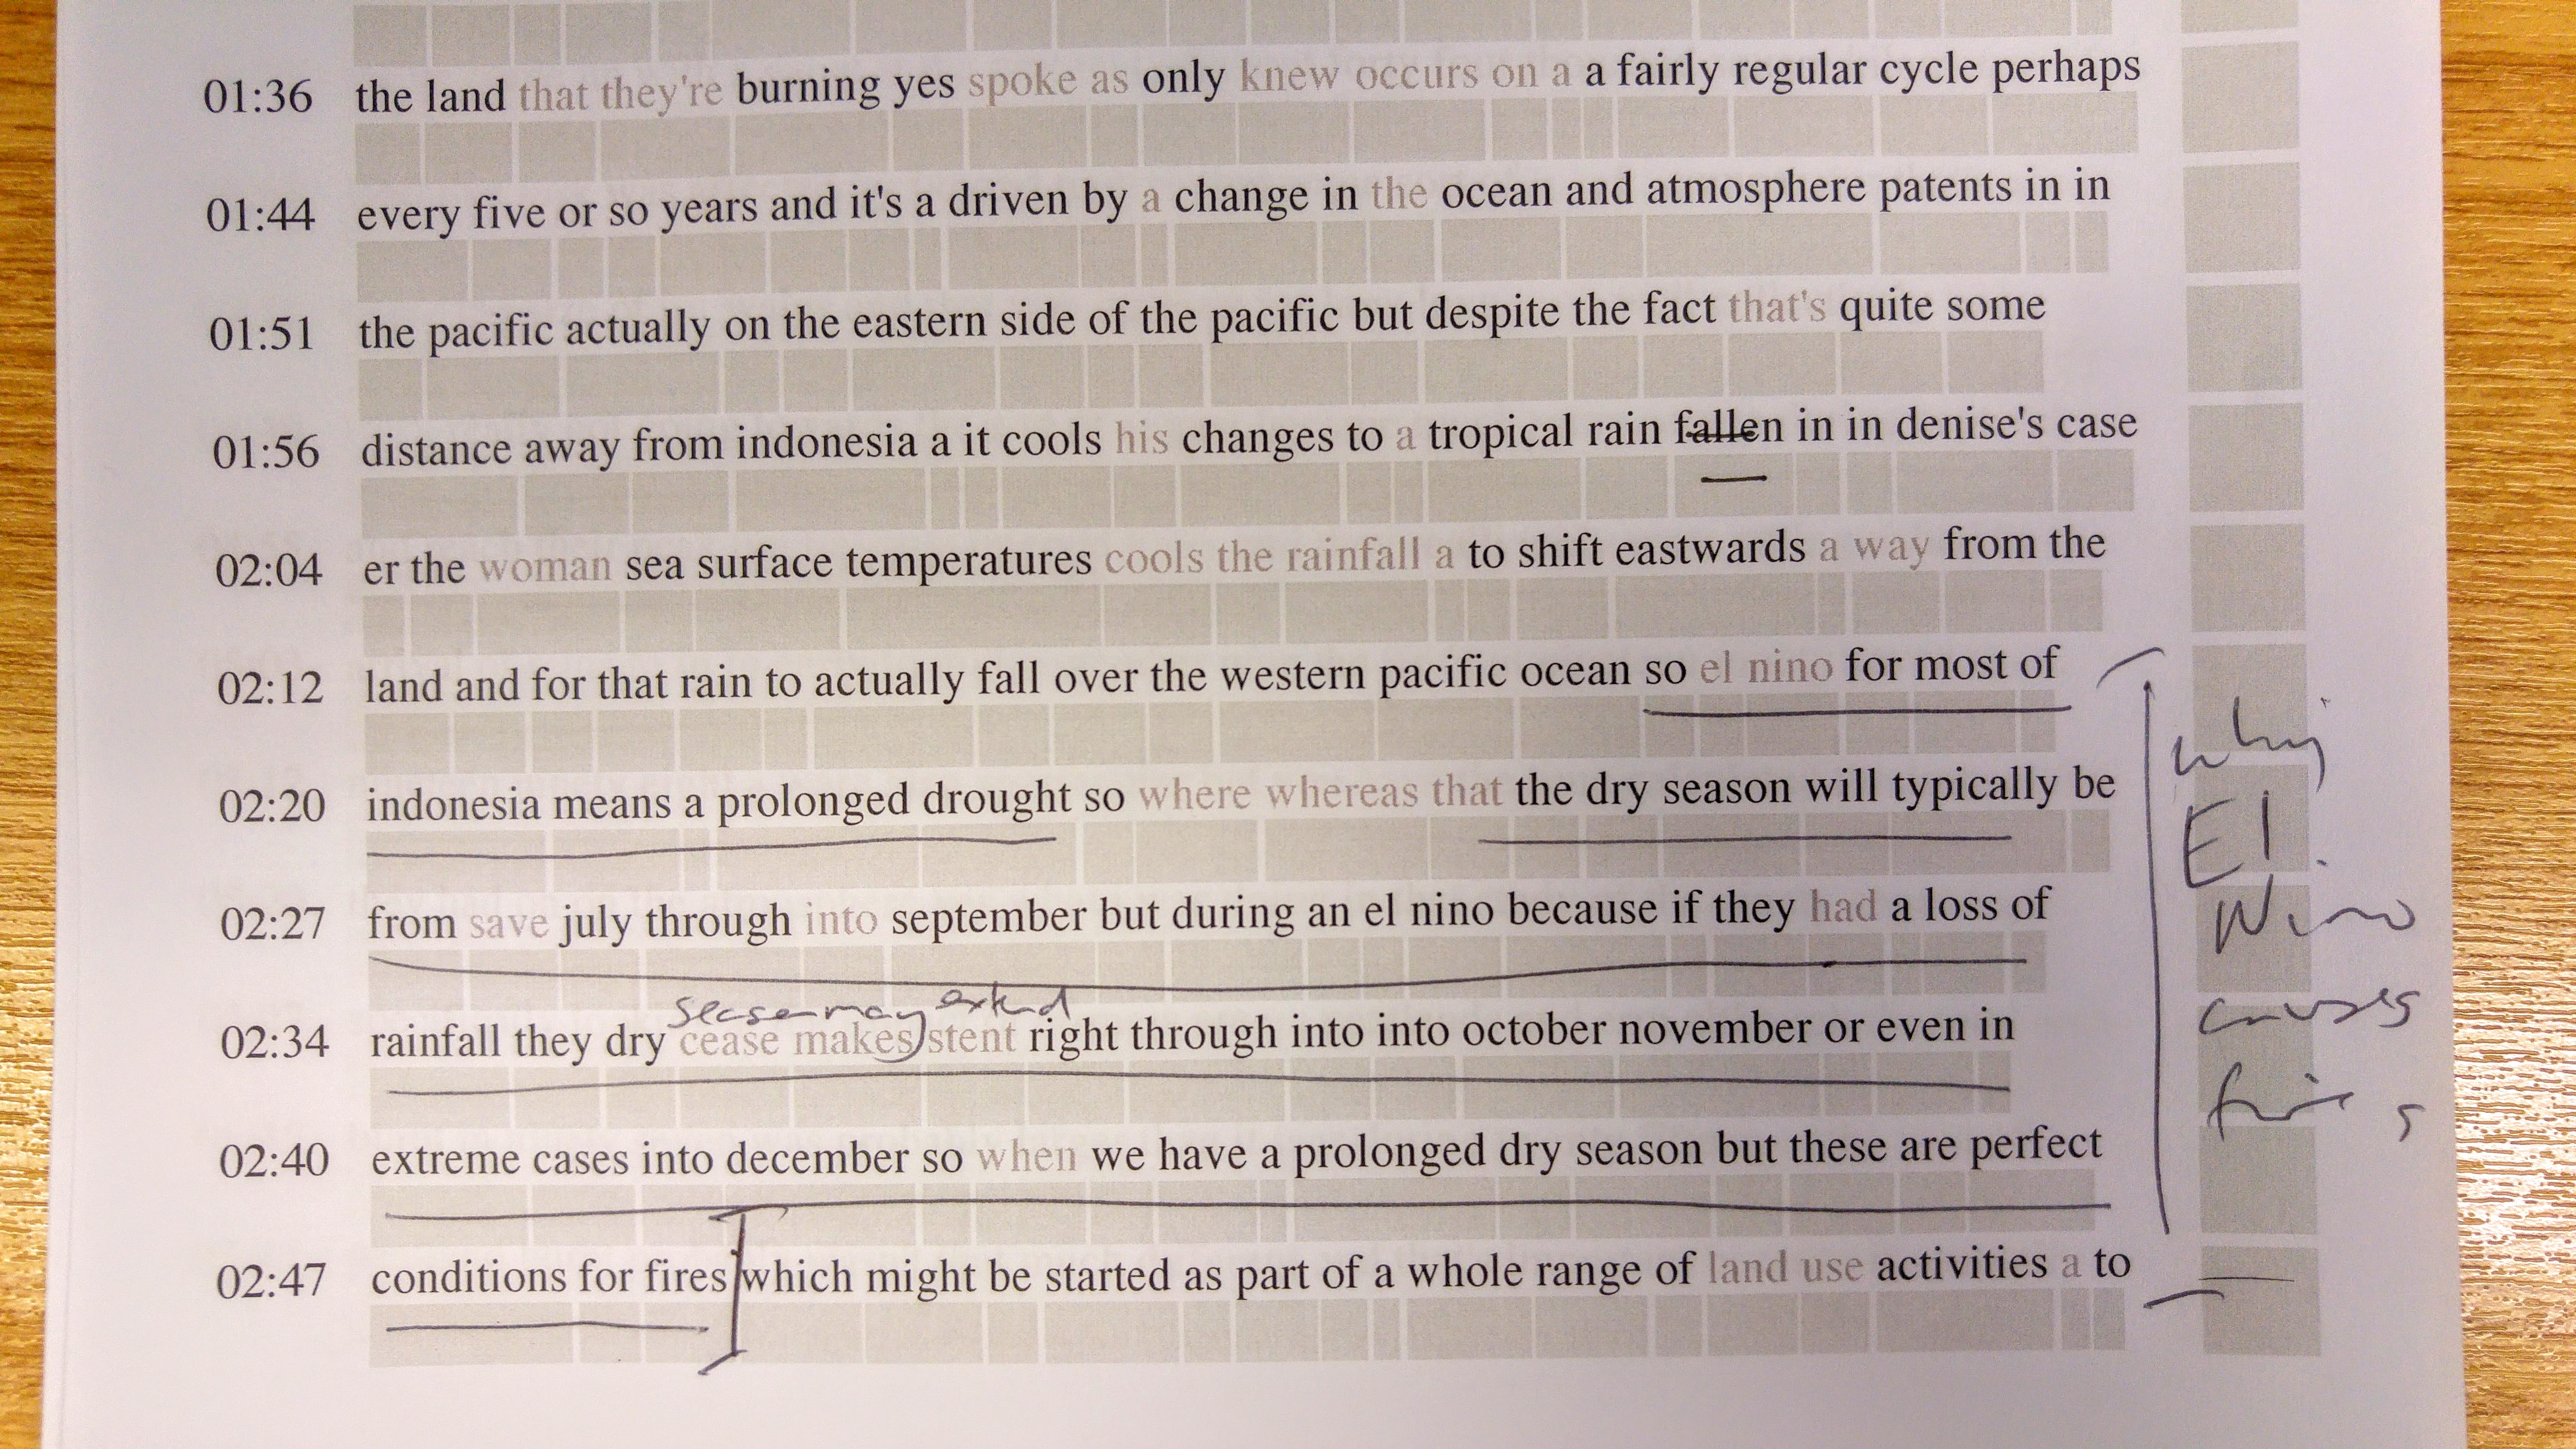
\includegraphics[width=\columnwidth]{figs/mockup}
  \caption{Paper prototype with natural annotations, including
    underlining, line down the side with notes, word corrections, and a
    vertical line to indicate the end of an edit.}
  \label{fig:natural}
\end{figure}

The transcript was printed double-spaced, with a grey box below each word to
indicate the underlining area.  Words with a low confidence rating were
`low-lighted' by shading them grey.  Each line of the transcript had a
timestamp on the left and a square box on the right, which could be used to
select a whole line at a time.

\subsection{Method}
We tested two inactive paper prototypes of the paper interface.
One used the speaker diarization information 
to segment the transcript into paragraphs, with the start of each paragraph
labeled with the speaker identifier in square brackets (e.g.
\texttt{{[}S1{]}}). The other version did not use any of this 
information. The users were presented with the normal transcript first,
followed by the one with speaker information.

For each version, we asked the participants to use a normal pen to annotate the
first page of the transcript as they would normally, to only use strikethrough
on the second page and only use underline on the third page. At the end of the
test, each participant was interviewed about their experience overall and
with each method.

\subsection{Results}
The reaction to the system was overwhelmingly positive. All of the
participants could immediately see the value of such a system and remarked that
it would save them significant amounts of time and \textit{``revolutionise''}
their production workflow.

\subsubsection{Natural behaviour}
The participants started the exercise by annotating the transcript any way they
wanted.  Three of the five participants used underlining to select desired
words, with one using strikethrough to remove words and the other using both
methods.  Three drew a line down the side of the page to select multiple lines
at a time.  Two used short vertical lines between words to signify in- and
out-points for edits.  Two corrected mistakes in the transcript by writing over
or above the incorrect word. Finally, one participant selected words using a
`lasso' technique.

Each participant used a different mixture of annotation techniques. Some of
these techniques, such as underlining, strikethrough and lines down the side,
are easy to detect.  Others, such as corrections, lasso and lines between
words, are less easy to detect. There was no room to write notes at the side of
the page, but one participant did it anyway and two others expressed an interest
in doing so if there was a margin. One participant said that they would
not want a margin.

\subsubsection{Additional features}
Four of the five participants found the paragraphs and speaker information
useful. Typically, interviews have a presenter and contributor and the
producers find it valuable to know when the presenter is asking a question.
Three of the participants said that they were able to find the questions much
more easily with this feature enabled. However, another participant said they
found the speaker diarization \textit{``distracting''}.

All participants found the timestamps and confidence shading features useful,
with some commenting that one timestamp per page would be sufficient.  All of
the participants liked being able to select whole lines at a time, with one
asking whether a similar function could be available to delete content. It was
also suggested that the side boxes could be used to rate or star a selection.

Four of the participants found the transcript was accurate enough to use for
editing their material.  The interview used by the other participant has a
strong Scottish accent which affected the transcript quality. Finally, several
participants noted the importance of listening to the recording and expressed a
desire to hear the content whilst reading the paper transcript.

\subsubsection{Select or delete}
The participants were asked whether
they preferred selecting or deleting words. Three of them preferred select, with
one commenting that it \textit{``felt more natural''} and another saying
deleting felt \textit{``counter-intuitive''}. The other two participants
preferred deleting, with one commenting that it was \textit{``the way my brain
  works''} and the other saying they prefer to \textit{``get stuff out of the
  way''}. As there was no agreement, the system should have options to cater
for a variety of translation methods.

%- Useful to know where presenter is asking question

%Diarization
%- Neal found it easier
  %- Shows where the questions are
%- Phil found it distracting
%- Wes found it absolutely useful
%- Marnie 'made it much easier', liked having paragraphs (usually one point per
%paragraph)


%Timestamps
%needed every couple of minutes

%Use L/R channels for presenter/contributor
%- Phil and Wes
%- Sometimes multiple on R channel (about one in eight interviews)

%Prefer landscape to portrait (landscape is `irritating' and doesn't match
%what's on screen)

%Whole line
%- Would like to delete line at a time

%Note-taking
%- One doesn't take many notes

%Correction
%- One corrects then selects edits
%- Wes would like option

%Highlighting
%- Asterix/star to mark important bits (Phil, Neal)
%- Underline twice (Neal, Marnie liked idea)
%- Wes sometimes double-stars

%Delete vs select (2 vs 3)
%- Phil likes to `get stuff out of the way'
  %- Words that aren't marked should be kept by default
  %- Underline should undo delete
%- Neal prefers selecting over deleting
  %- Delete should undo select, if underlined too far
%- Wes prefers selecting - deleting is `counter-intuitive'
  %- Would like delete to override select, but would like options for opposite
%- Marnie found it trickier to delete than select, selection is more natural
  %- worried about deleting something good
%- Alex feels delete is more natural, 'way may brain works, 'challenge is to
%nibble away', thinks delete should be active, select should override delete

%Margin
%- Phil wouldn't need a margin
%- Neal would like one

%Export
%- gaps should be put between edits (real-time?)

%Transcript
%- Phil and Neal no problems
%- Wes had problems (strong Scottish accent) made it unusable

%Observation
%- Neal
  %- underlined as he read (unprompted), scribbled out when mistake made
  %- found it more difficult to only delete
%- Wes
  %- vertical lines for in/out points

%Other
  %- Neal would like to press and hear word (on laptop?)
    %- Wes: Don't know what sounds good
  %- Wes works in a team of 3/4. They use Box to collaborate

\subsection{Discussion}
%Our system performs the same function as these systems, but uses a paper
%interface rather than a screen-based one.
%Our system
%similarly interprets the paper annotations and applies them to the media
%content.
%Our system does not yet have the ability to replay content from the
%paper interface, but this is a feature that could later be included.
%Our system is based on printed transcripts rather than video frames on
%a tablet, but approaches the same problems from a different angle.
%These systems do not provide the user with any pre-written notes.
%Our system uses speech-to-text to generate a transcript, which the user can
%then annotate further.
The participants used a variety of techniques to annotate the transcripts, 
but underline, strikethrough and lines down the side were common. There were
strong but mixed opinions on whether selection of desired material, or removal
of unwanted material, was the best approach to use for editing, so both should
be made available where possible. However, it is still not clear what should
happen when underline and strikethrough are used together, and which should
override the other.

The transcripts were generated using speech-to-text but were considered good
enough to edit with. We found that participants enjoyed having paragraphs, speaker
information, timestamps, confidence shading and being able to select whole lines.

Some participants expressed a desire to listen to the media
from the paper interface, and this functionality has been shown to be useful
in previous work. Users could start playback by pressing a word with the
digital pen. This could be achieved either by wirelessly
linking the digital pen to a computer that plays the content, or by storing
the audio on the pen itself similarly to the LiveScribe Sound
Stickers\footnote{\url{http://store.livescribe.com/sound-stickers-1-1.html}}.

Previous work has also shown the benefits of being able to write freehand notes
which link to specific points in recordings. These could be attached to a
screen-based interface similarly to ProofRite \citep{Conroy2004}, or handwriting
recognition could be used to store and organise these notes in a structured
way. This approach could also be used to fix incorrect words in the transcript.

Media content is often produced in teams rather than individually.  Although
our system does not prevent multiple people from working on a transcript, it
does not exploit opportunities to smoothly handle multiple users.

We will shortly be conducting a formal evaluation of our system at the BBC
where it will be used to produce audio and video content for broadcast. 

%Providing a function to align an existing script to the recording would allow
%this functionality to be used with scripted programmes.

\subsection{Conclusion}
In this paper, we presented a novel system for editing media content using a
paper-based interface. We tested this concept using a paper prototype in an
informal test on five radio producers.

The participants all reacted very positively to the system. They enjoyed the
additional features we tested including speaker information, paragraphs,
timestamps, confidence shading and selection of whole lines. Based on their
feedback, we also added an optional margin to the interface.

A variety of annotation marks were used by the participants to indicate edit
decisions, including underline, strikethrough, lines down the side and lines
between words.  Participants either preferred to select content they wanted or
to delete content they didn't want, and felt strongly either way.

There are a number of opportunities to build on the system, including being
able to capture freehand notes, listen to the content using the paper
interface, fix incorrect words and work collaboratively.

\section{System design}
Using the feedback from producers, we designed and created a working prototype
of the system (see Figure~\ref{fig:diagram}). To build our prototype, we
collaborated with Anoto who are the manufacturers of the digital pen. We
developed the interface, speech-to-text and media editing, whilst Anoto
handled the transcript printing and translation of the annotations to edit
commands. 

\begin{figure}[h]
  \centering
  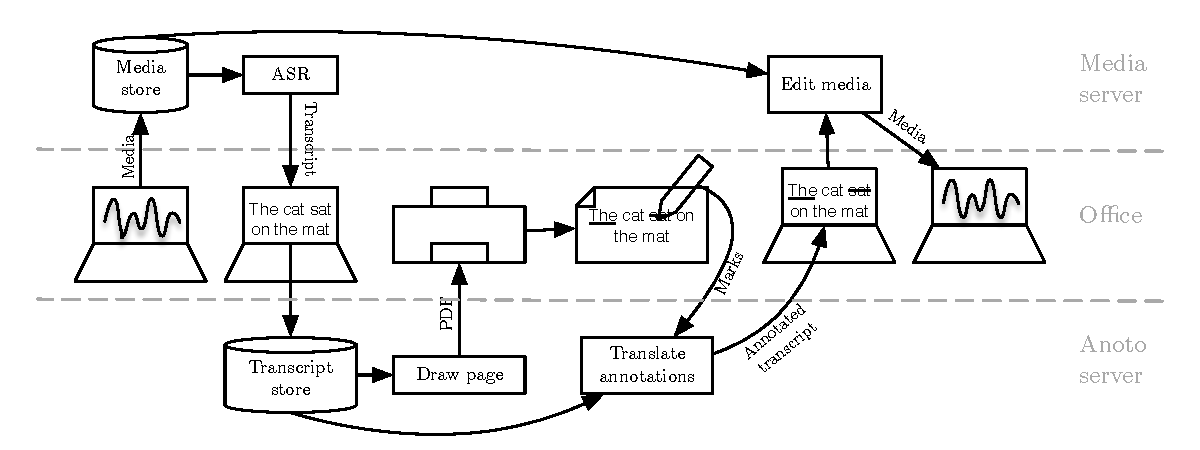
\includegraphics[width=\columnwidth]{figs/uist-sys-diagram}
  \caption{System diagram, flowing from top to bottom}
  \label{fig:diagram}
\end{figure}

Based on the feedback from users, the timestamps, paragraphs, speaker
information and confidence shading have been retained. However the timestamps
only appear at the start of each paragraph. An optional margin has also been
added to allow users to make unstructured notes using their digital pen. 
It is not currently possible to select a whole line at a time, but this will
shortly be added.

For each word in the transcript, two rectangular active areas are defined on
the page -- one around the word itself and another in the space directly below
the word, which is lightly shaded. Any marks made on or below the word label
that word as `deleted' and `selected', respectively. This allows the user to
use a digital pen to delete words using a strikethrough, or to select words by
underlining.  The annotations are automatically uploaded in batch to the system
when the pen is docked.

\begin{figure}[h]
  \centering
  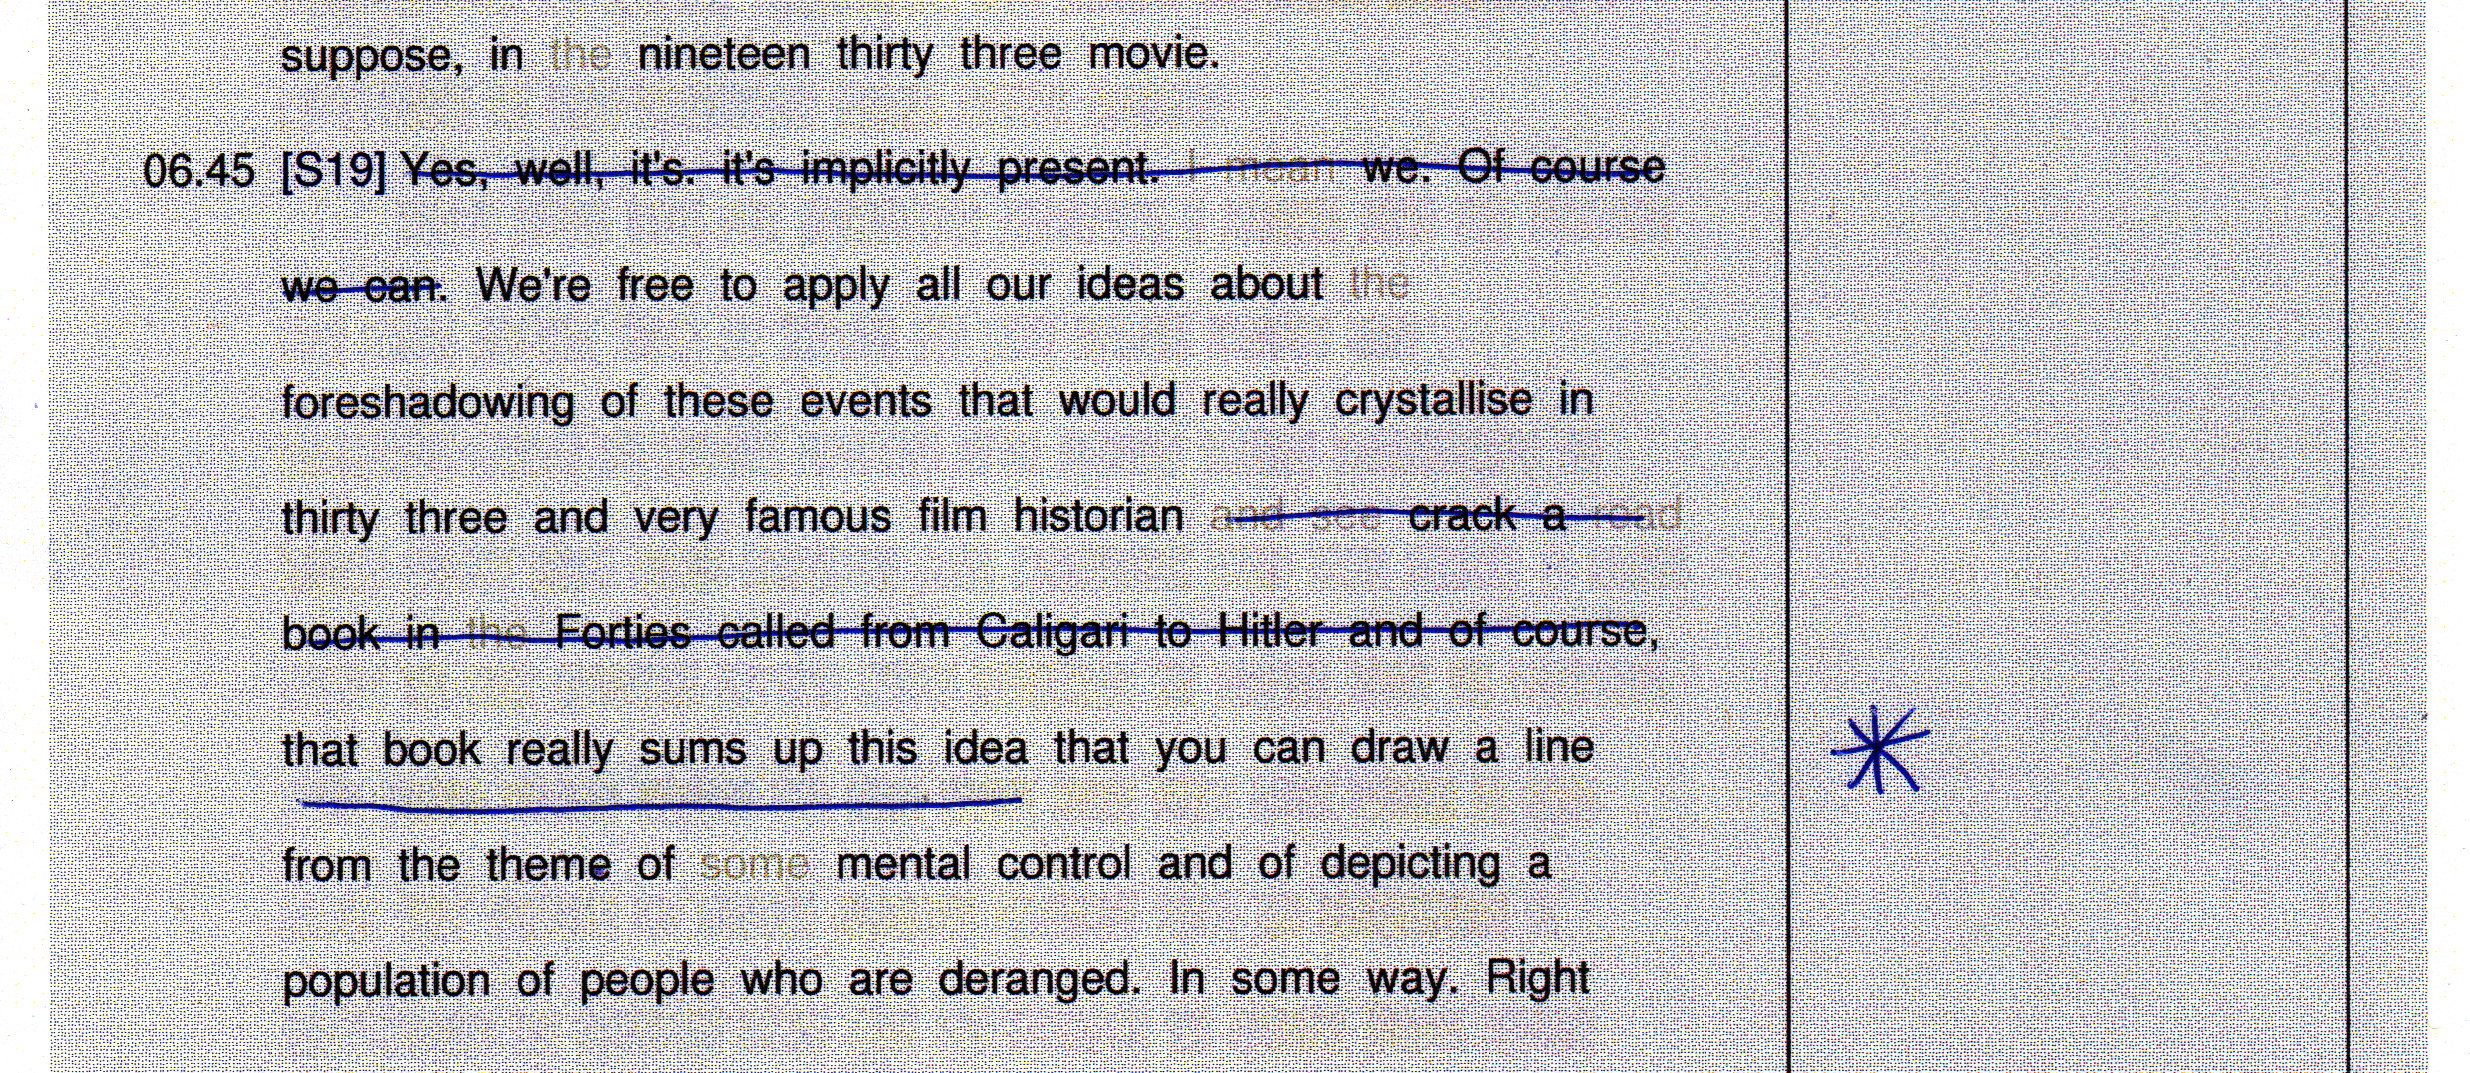
\includegraphics[width=\columnwidth]{figs/interface-darkened}
  \caption{Example of working prototype, showing the shaded box beneath each
    word, paragraph for each speaker with timestamp (06.45) and identity (S19),
    and optional margin for freehand annotations.}
  \label{fig:layout}
\end{figure}

The uploaded annotations are combined with the word timings to calculate the
edit commands.  These can be used to directly edit the media (as shown in
Figure~\ref{fig:diagram}) which removes the unwanted parts of the content. This
is known as a `destructive' edit.  Alternatively, the edit commands can be used
to create an edit decision list (`EDL'). An EDL file describes the in- and
out-point for a series of edits, which can be loaded into audio or video
editing software.  As it is `non-destructive', this approach allows the user to
make corrections to the edit before it is rendered. 

%Several approaches can be taken in interpreting the delete and
%select annotations:
%\begin{itemize}
  %\itemsep0em
  %\item Remove words marked as deleted, except those marked as selected
  %\item Only keep words marked as selected, except those marked as deleted
  %\item Remove words marked as deleted, highlight words marked as selected
%\end{itemize}

\section{Methods}

\subsection{Design and procedure}

% Explain why video recording wasn't used

\paragraph{Stage 1: Training and usability study}
Firstly, the participant will be briefed on the background, objectives and
design of the study as detailed in the protocol.  Should they wish to
participate, they will be asked to read and agree to the consent form.

There are two objectives to the training stage – firstly to introduce the
participant to the prototype system so that they understand its capabilities,
and secondly to test the usability of the interface.

The experimenter will set the participant up on the prototype system, including
giving them access to the web-based interface, giving them a digital pen and
configuring the pen’s docking system. The participant will then receive
training on how to operate the web interface, print out transcripts correctly
and use the pen.

The participant will then be asked to perform a series of typical tasks. The
participant can ask questions and, if they become stuck, the experimenter can
prompt them. However, the experimenter will not give any other directions. The
experimenter will note whether the participant was able to successfully
complete the task and document any problems or confusion experienced during the
execution of the tasks. This process will help to flag any obvious stumbling
blocks.

\paragraph{Stage 2: Observation}

This stage will involve observing the participant editing two pieces of content
- one using the screen-based interface and the other using the paper-based
interface. The order of the observation will be alternated between
participants. The two pieces of content should be similar in nature, but
different so that the participant isn't already familiar with the content.

The observation will be done passively to allow natural interaction with the
system in the participant's normal work environment. The experimenter will sit
beside them making written notes. When the participant has some 'down-time',
the experimenter may choose to ask some questions in order to verify or clarify
something they have observed.

The specific items of interest at this stage include:
\begin{itemize}
\item Editing workflow
\item Tools used
\item Data generated
\item Usability challenges and problems
\item Navigation and edit actions
\item Time taken to complete tasks
\item Unexpected reactions
\item Unanticipated usage
\end{itemize}

The prototype will be configured to electronically log the actions of the
participant, which will help provide insights into usage of the various
features of the prototype.

Software Usability Scale \citep{Brooke1996}
Perceived Usefulness \citep{Davis1989}

With the participant's permission, photos may be taken of paper notes,
annotations or the work environment (see 'data protection' section below).

\paragraph{Stage 3: Interview}
Following the observation stage, the participant will be left with access to
the prototype system for at least a further week. This will give them the
opportunity to use the system as part of their day-to-day work and uncover
issues which may be appear in the observation.

After this period has passed, the participant will be interviewed about their
experience. The primary objective is to compare the two production methods and
extract the advantages and disadvantages of both.

An audio recording will be made of the interview (see 'data protection' section
below). This will allow the participant to speak their mind and allow the
experimenter to give the participant their full attention whilst capturing all
of the provided information.

The questions asked will include:
\begin{itemize}
\item Which aspects of the screen-based system did you / did you not find useful?
\item Which aspects of the paper-based system did you / did you not find useful?
\item Overall, which system did you prefer and why?
\end{itemize}


\subsection{Participants}
To make the most of the principal investigator's position in the BBC,
participants will be recruited exclusively from the BBC. They will be invited
to volunteer by way of email passed around using existing contacts in various
departments that produce speech-based content. 

The nature of the study requires that participants conduct the tasks as part of
their day-to-day job. Therefore, participants will be required to gain
permission from their line manager to take part.

Programmes and producers vary significantly in genre and production techniques.
To take this into account, participants will be recruited so that there is a
representative range of styles.

\subsubsection{Selection criteria}

\begin{itemize}
\item The programme being created should be speech-based.
\item The content of the programme must not contain any sensitive material, as
the transcription will be sent to a third-party for transcription (see 'data
protection' section below).
\item The turn-around time of the programme must be long enough to allow time
to recover from any technical issues without affecting broadcast output.
\item The participant must have permission from their line manager to take part.
\end{itemize}

The study will involve between six and nine participants, depending on how many
meet the criteria. This should uncover over 90\% of usability problems
\citep{Nielsen1993} whilst covering a range of genres and styles, and being a
manageable number given the duration of the experiment.

The study will take place at the participant's own desk at their normal place
of work. As the prototype is web-based, they can use their own computer. There
is a standard configuration for BBC desktop computers, so the environment
should be similar for each participant. Use of display screen equipment is
already covered under the existing BBC risk assessment process.

\subsection{Analysis}

\section{Study results}

\subsection{Qualitative analysis}

% MAIN TOPICS:
% Annotation
% Correction
% Editing
% Listening
% Normal workflow
% Paper admiration/restrictions/waste
% Screen-based working/reading paper
% Transcript accuracy
% Transcript itself


% OTHER TOPICS:
% Collaboration
% Cost
% Custom vocab
% Digital/analogue
% Combining recordings
% Non-linear workflow
% Pen hardwaare
% Working remotely
% Speaker diarization
% Speed
% Structuring thoughts
% Transcription speed
% Translation


\subsection{Metrics}

% Speed

\begin{figure}[h]
  \centering
  \begin{tikzpicture}
  \begin{axis}[
    legend pos=outer north east,
    legend cell align=left,
    xmin=0,
    ymin=0,
    xlabel={Audio length (mins)},
    ylabel={Edit time (mins)}]

  % NORMAL
  \pgfplotstableread{
    X Y
    30 30
    58 43
    32 23
    35 53
    28 35
    28 32
  }\normaltimes
  \addplot [only marks, mark = *, red] table {\normaltimes};
  \addlegendentry{Normal results}
  \addplot [thick, red] table[
      y={create col/linear regression={y=Y}}
  ]{\normaltimes};
  \addlegendentry{Normal trend}

  % SCREEN
  \pgfplotstableread{
    X Y
    37 24
    61 61
    30 30
    25 49
    26 31
    41 28
  }\screentimes
  \addplot [only marks, mark = square*, blue] table {\screentimes};
  \addlegendentry{Screen results}
  \addplot [thick, dotted, blue] table[
      y={create col/linear regression={y=Y}}
  ]{\screentimes};
  \addlegendentry{Screen trend}

  % PEN
  \pgfplotstableread{
    X Y
    12 9
    75 56
    31 17
    22 19
    27 27
    38 37
  }\pentimes
  \addplot [only marks, mark = diamond*, green] table {\pentimes};
  \addlegendentry{Pen results}
  \addplot [thick, loosely dashed, green] table[
      y={create col/linear regression={y=Y}}
  ]{\pentimes};
  \addlegendentry{Pen trend}

  \end{axis}
  \end{tikzpicture}
  \caption{Edit time performance for each editing system}
  \label{fig:penedittime}
\end{figure}

% Usefulness


% Usability




\section{Discussion}

\section{Conclusions}

\section{Future work}
